\section{Auswertung}
\label{sec:Auswertung}

%\begin{figure}
%  \centering
%  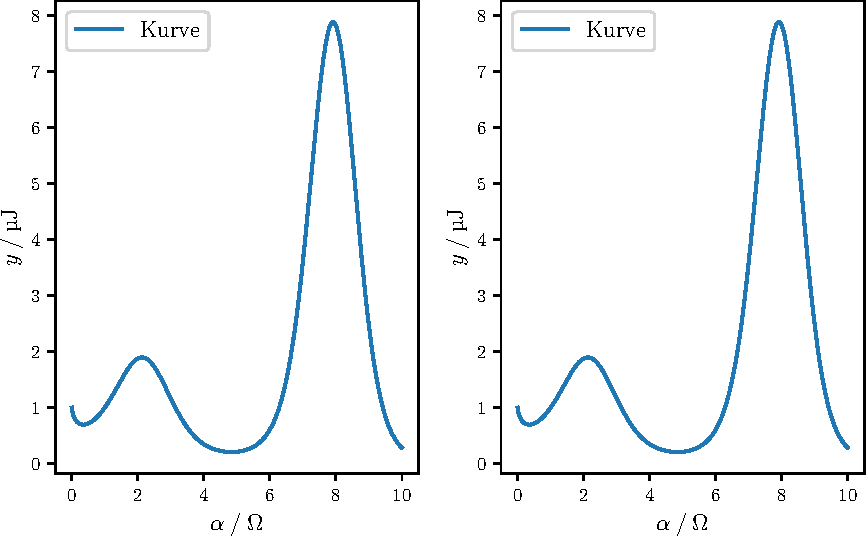
\includegraphics{plot.pdf}
%  \caption{Plot.}
%  \label{fig:plot}
%\end{figure}


Zuerst wird die Erfüllung der Bedingung $2 \cdot v_0 = v_{auf} - v_{ab}$ geprüft, um Werte, bei denen die Randbedingungen
des Experiments nicht erfüllt wurden, zu verwerfen. Es wird im folgenden nur mit den Messwerten weitergearbeitet, bei denen die 
prozentuale Abweichung vom Sollwert bei unter 50\% liegt. Sie sind in der \autoref{tab:geschw} gekennzeichnet. \\
Die Geschwindigkeiten in \autoref{tab:geschw} wurden via $v = \frac{s}{t}$ aus den gemessenen Zeiten errechnet.\\

\begin{table}[H]
  \centering
  \caption{Die Differenzen der Auf- und Abtriebsgeschwindigkeiten sowie die Ruhegeschwindigkeit der Öltröpfchen sowie ihre relative Abweichung vom Sollwert nach der Ruhegeschwindigkeit.}
  \begin{tabular}{ccccc}
    \toprule
    {$T  \mathbin{/} \; ° \unit{\celsius}$} &
    {$\mathbin{Spannung} \; \; U  \mathbin{/} \unit{\volt}$} &
    {$2 \cdot v_0 \mathbin{/} \mathbin{div / s}$} &
    {$v_{auf} - v_{ab} \mathbin{/} \mathbin{div / s}$} &
    {Abweichung $\mathbin{/} \unit{\percent}$}\\
    \midrule
21 & 4,57 &   -0,06  & 0,09  &  166,66 \\
21 & 4,57 &   -0,26  & 0,07  &  471,43 \\
21 & 4,57 &   -0,41  & 0,11  &  472,30 \\
21 & 4,57 &   0,12   & 0,21  &  \textbf{42,86}\\
21 & 4,57 &   -0,17  & 1,74  &  110,00\\
21 & 3,97 &   0,25   & 0,15  &  66,66\\
21 & 3,97 &   0,30   & 0     &  ungültig\\
21 & 3,97 &   -0,27  & 0,09  &  400,00\\
21 & 3,97 &   -0,17  & 0,13  &  230,77\\ 
21 & 3,97 &   -0,12  & 0,13  &  192,30\\
22 & 3,04 &   -0,24  & 0,04  &  700\\
22 & 3,04 &   0,13   & 0,23  &  \textbf{43,48}\\
22 & 3,04 &   0,26   & 0,14  &  85,71\\
22 & 3,04 &   0,32   & 0,13  &  146,15\\
22 & 3,04 &   -0,22  & 0     &  ungültig\\
23 & 4,91 &   0,65   & 0,09  &  622,22\\
23 & 4,91 &   0,29   & 0,10  &  190,00\\
23 & 4,91 &   -0,44  & 0,87  &  150,57\\
23 & 4,91 &   0,15   & 0,11  &  \textbf{36,36}\\
23 & 4,91 &   0      & 0,11  &  100,00\\
23 & 2,20 &   0,07   & 0,09  &  \textbf{22,22}\\
23 & 2,20 &   0,17   & 0     &  ungültig \\
23 & 2,20 &   -0,27  & 0,15  &  280,00\\
23 & 2,20 &   -0,23  & 0     &  ungültig\\
23 & 2,20 &   0,07   & 0,13  &  \textbf{44,00}\\

    \bottomrule
  \end{tabular}
  \label{tab:geschw}
\end{table}




\subsection*{Bestimmung der Elementarladung}

Für das elektrische Feld des Plattenkondensators wird die Formel
\begin{equation}
  E = \frac{U}{d}
\end{equation}
genutzt.\\
Es wird mit den Konstanten 
\begin{eqnarray}
  \rho_{Öl} = 886 \mathrm{\frac{kg}{m^3}}\\
  \rho_{Luft} = 1,16 \mathrm{\frac{kg}{m^3}}\\
  g = 9,81 \mathrm{\frac{m}{s}} \\
  d = (7,6250 \pm 0,0051) \mathrm{mm}
\end{eqnarray}
gerechnet, die bei Durchführung des Versuchs gegeben waren. \\

Nach xxxxx wird aus den berechneten Geschwindigkeiten der Radius
der Tröpchen bestimmt. Aus dem Radius wird durch xxxx die Ladung der Tröpchen berechnet und nach Cunningham korrigiert. \\
So ergeben sich die Werte in xxxx.\\

\begin{table}[H]
  \centering
  \caption{Die berechneten Radien, unkorrigierten und korrigierten Ladungen der Öltröpfchen.}
  \begin{tabular}{ccccccc}
    \toprule
    {$T  \mathbin{/} \; ° \unit{\celsius}$} &
    {$\mathbin{Spannung} \; \; U  \mathbin{/} \unit{\volt}$} &
    {$2 \cdot v_0 \mathbin{/} \mathbin{div / s}$} &
    {$v_{auf} - v_{ab} \mathbin{/} \mathbin{div / s}$} &
    {Radius $r \mathbin{/} \unit{\metre} \cdot 10^{-7}$} &
    {unkorrigierte Ladung $q \mathbin{/} \unit{\coulomb}}$} &
    {korrigierte Ladung $q \mathbin{/} \unit{\coulomb}}$} \\
    \midrule
    21 & 4,57 &   0,12   & 0,21  &  42,86  &  x & x  \\
    22 & 3,04 &   0,13   & 0,23  &  43,48  &  x & x  \\
    23 & 4,91 &   0,15   & 0,11  &  36,36  &  x & x  \\
    23 & 2,20 &   0,07   & 0,09  &  22,22  &  x & x  \\
    23 & 2,20 &   0,07   & 0,13  &  44,00  &  x & x  \\
    \bottomrule
  \end{tabular}
  \label{tab:geschw}
\end{table}



